\chapter{不安定物体を支持可能な群ロボットシステム}
本章では,まず提案する不安定物体を支持可能な群ロボットシステムについて説明する.
次に,システムのモデリングについて説明する.

%--------------------------------------------------------------
\section{システムの提案}
本研究の提案する自身の体で不安定な物体を支持し運搬する群ロボットシステムを実現するために,ロボット群が搬送物体を支持する支持部とシステム全体を移動する移動部に分ける必要がある.

また,ロボットの台数は限られているので,支持部のロボットの台数が多いほど,物体を安定に支持できるが,移動部に負担がかかるため,全体の移動速度が遅くなることが考えられる.一方,移動部に関しては,ロボットが多いほど,全体の速度は速いが,支持部のロボットが少ないため,物体が倒れる可能性がある.

本研究の最終目標として,支持部と移動部の間のトレードオフを考慮し,最適の割合でロボット群にタスクを割り当てる必要がある.今回の研究はその前段階として,支持部のロボットが物体を支えるための条件を検討する.
\section{問題設定}
環境・ロボット・運搬対象物に関する前提条件は以下の通りとする.
\begin{itemize}
    \item 環境
    \begin{itemize}
        \item 平面
    \end{itemize}
    \item ロボット
    \begin{itemize}
        \item 前後移動可能
        \item 物体を両側から支持して運搬する
        \item 支持と移動の役割を分担させる
        
    \end{itemize}
    \item 運搬対象物
    \begin{itemize}
        \item 左右だけに倒れる長方形
        \item 重心位置,物体位置は既知
        \item 初期姿勢からの傾きの許容範囲は±5deg未満
    \end{itemize}
    
\end{itemize}
\section{システム全体のモデル}
物体が倒れるときや物体を支持するための条件を検討するために,システムのモデリングを行う.そのモデリングの概要について述べる.モデリングした図を\reffig{modeling}に示す.ここで,縦長い物体を真ん中に立てて,その両側に長方形のロボットが置いてある.ロボット1とロボット2は左と右にそれぞれ置く.また,これらを移動部の上に乗せた.今回移動部は地面との摩擦を無視できる横長い台車と仮定し,ロボットと物体の間の抗力は中央に作用すると仮定する.\reffig{freebody}に物体に作用する力の図を示す.ここで,物体に重力による力,ロボットと台車からの垂直抗力,ロボット・台車との摩擦が作用する他に,台車に力をかけた場合の物体にそれと逆向きに慣性力$F^{\prime}$が働く.また,ロボット1とロボット2の寸法は同じなので,$h_{r_1}=h_{r_2}=h_{r}$とする.
本稿におけるモデリングに使用した変数を\reftab{model-parameter}に示す.

\begin{figure}[tb]
 \centering
  \begin{tabular}{c}
   
   \begin{minipage}{0.5\hsize}
    \centering
     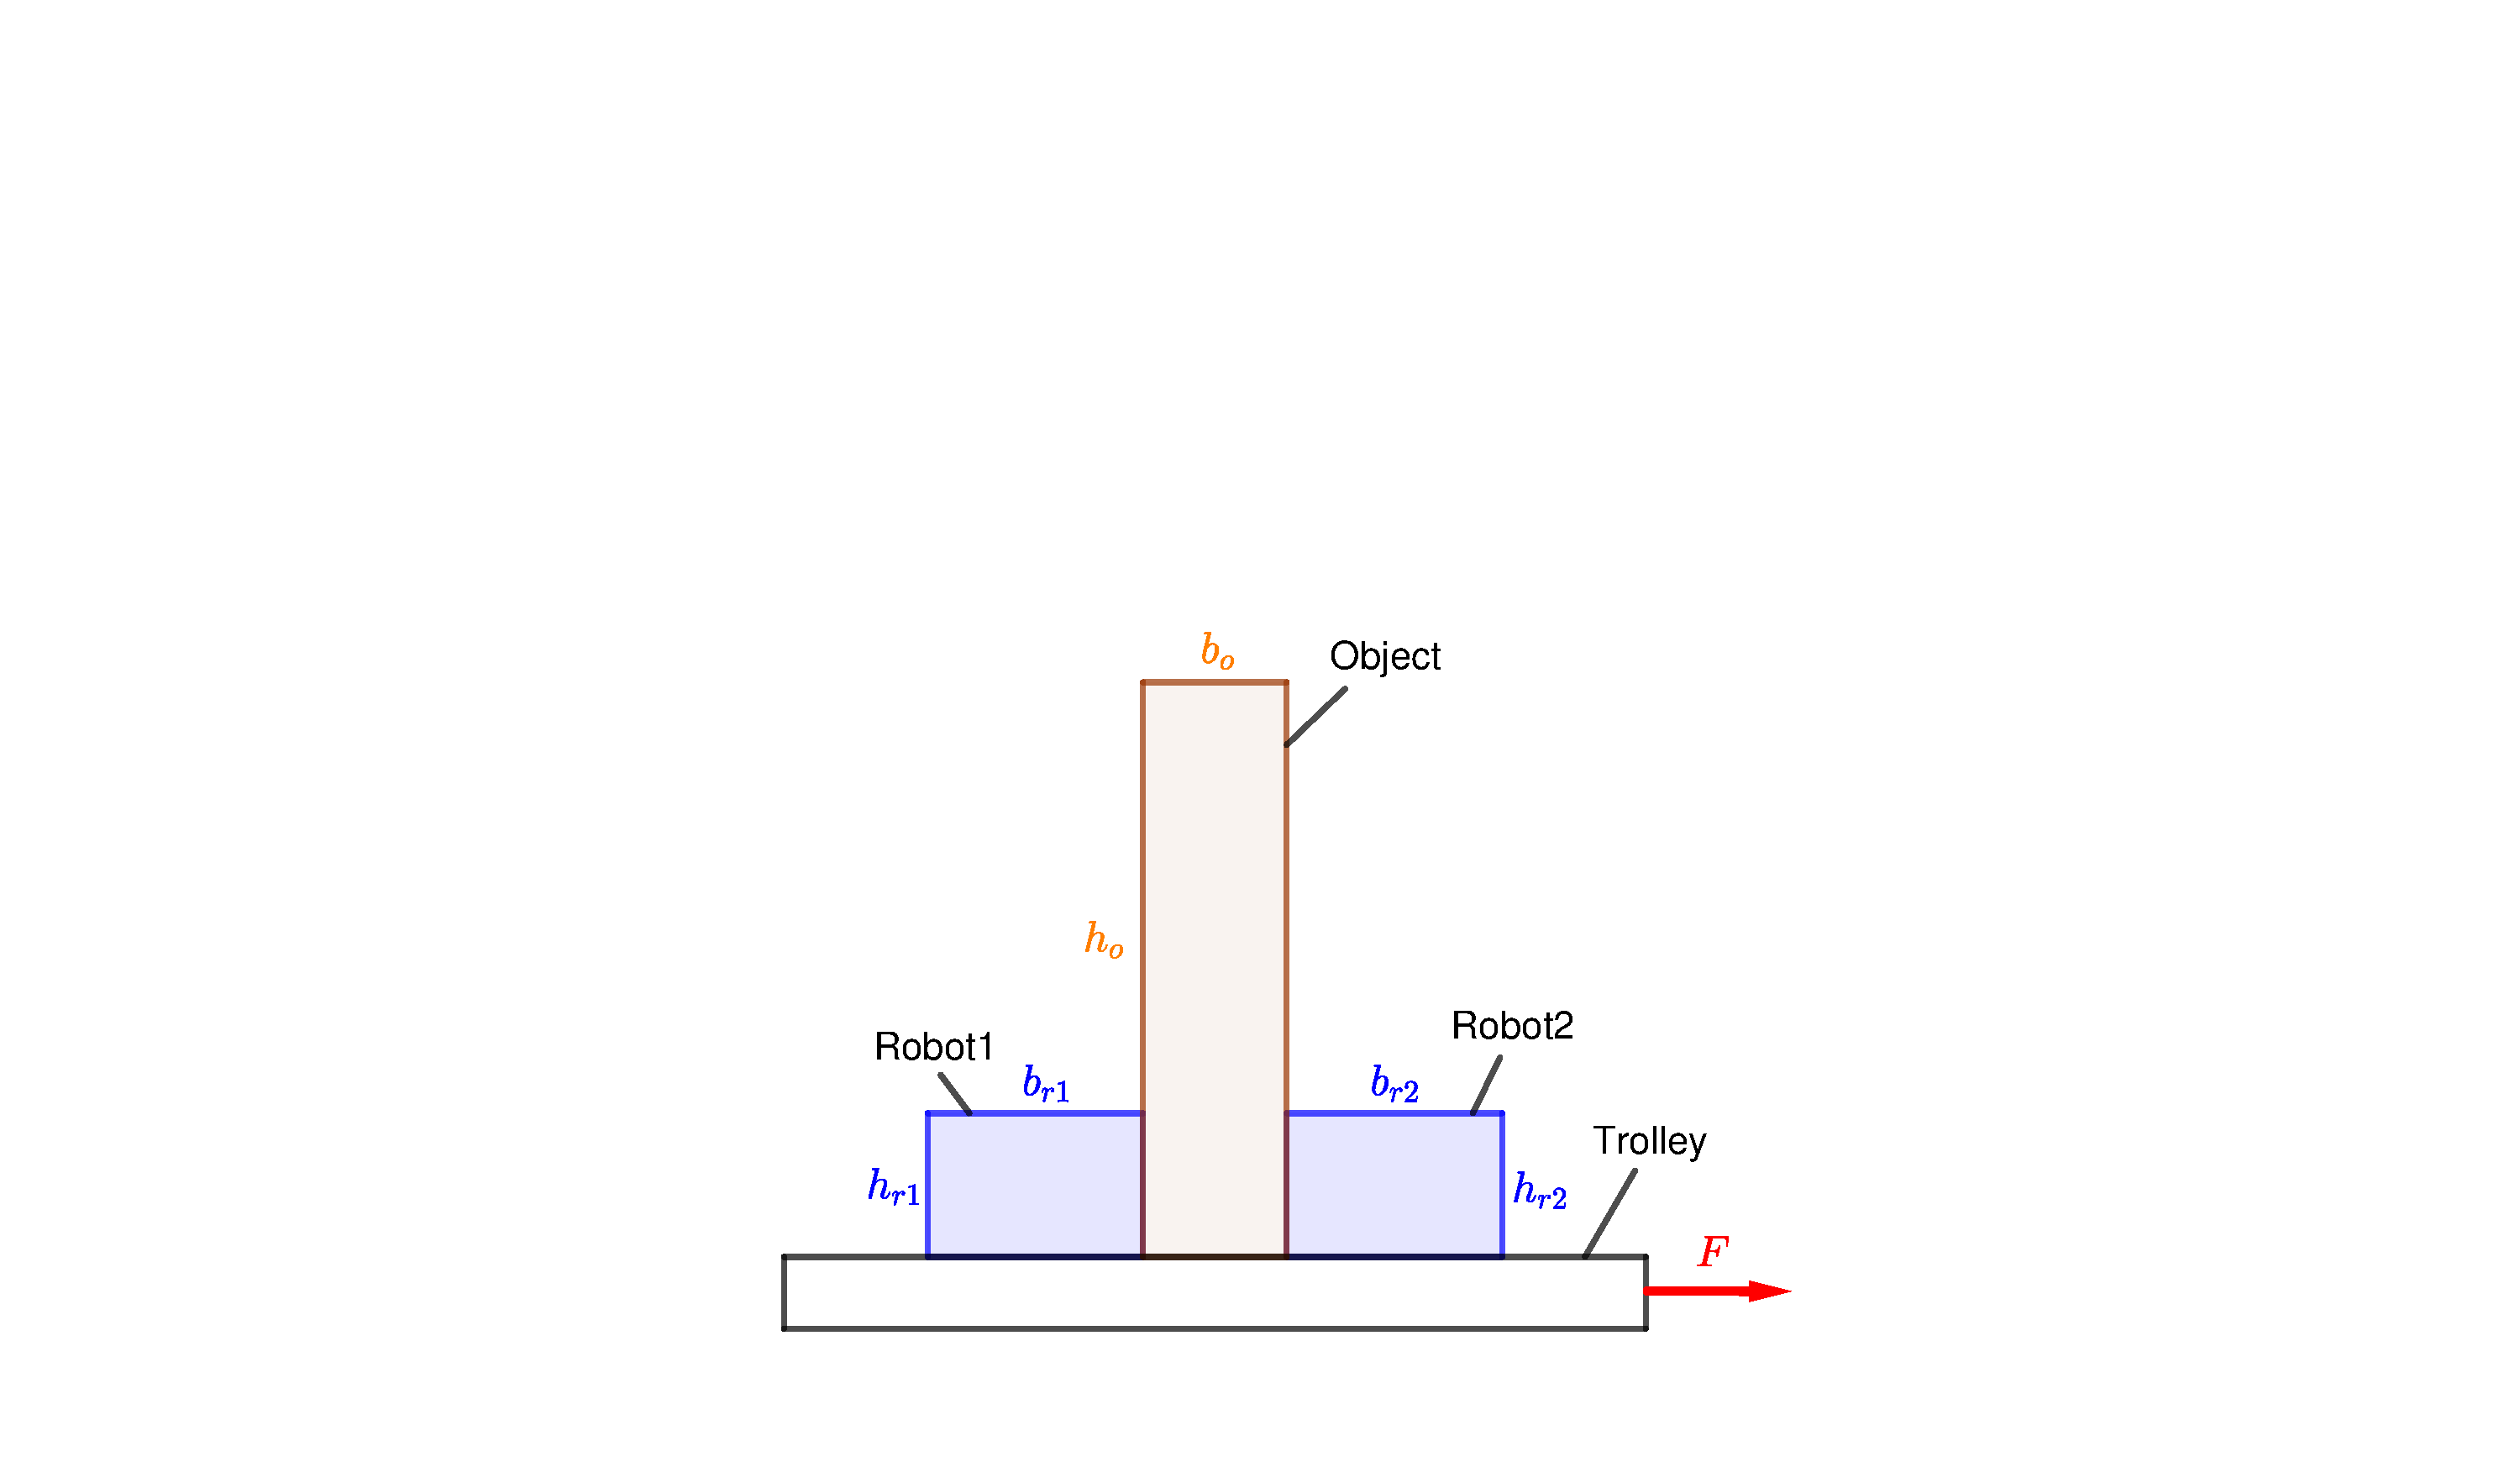
\includegraphics[trim=0 0 0 15, clip,width=\columnwidth]{./figure/model.pdf}
     \caption{Simplified model}
     \labfig{modeling}
   \end{minipage}
   
   \begin{minipage}{0.5\hsize}
    \centering
     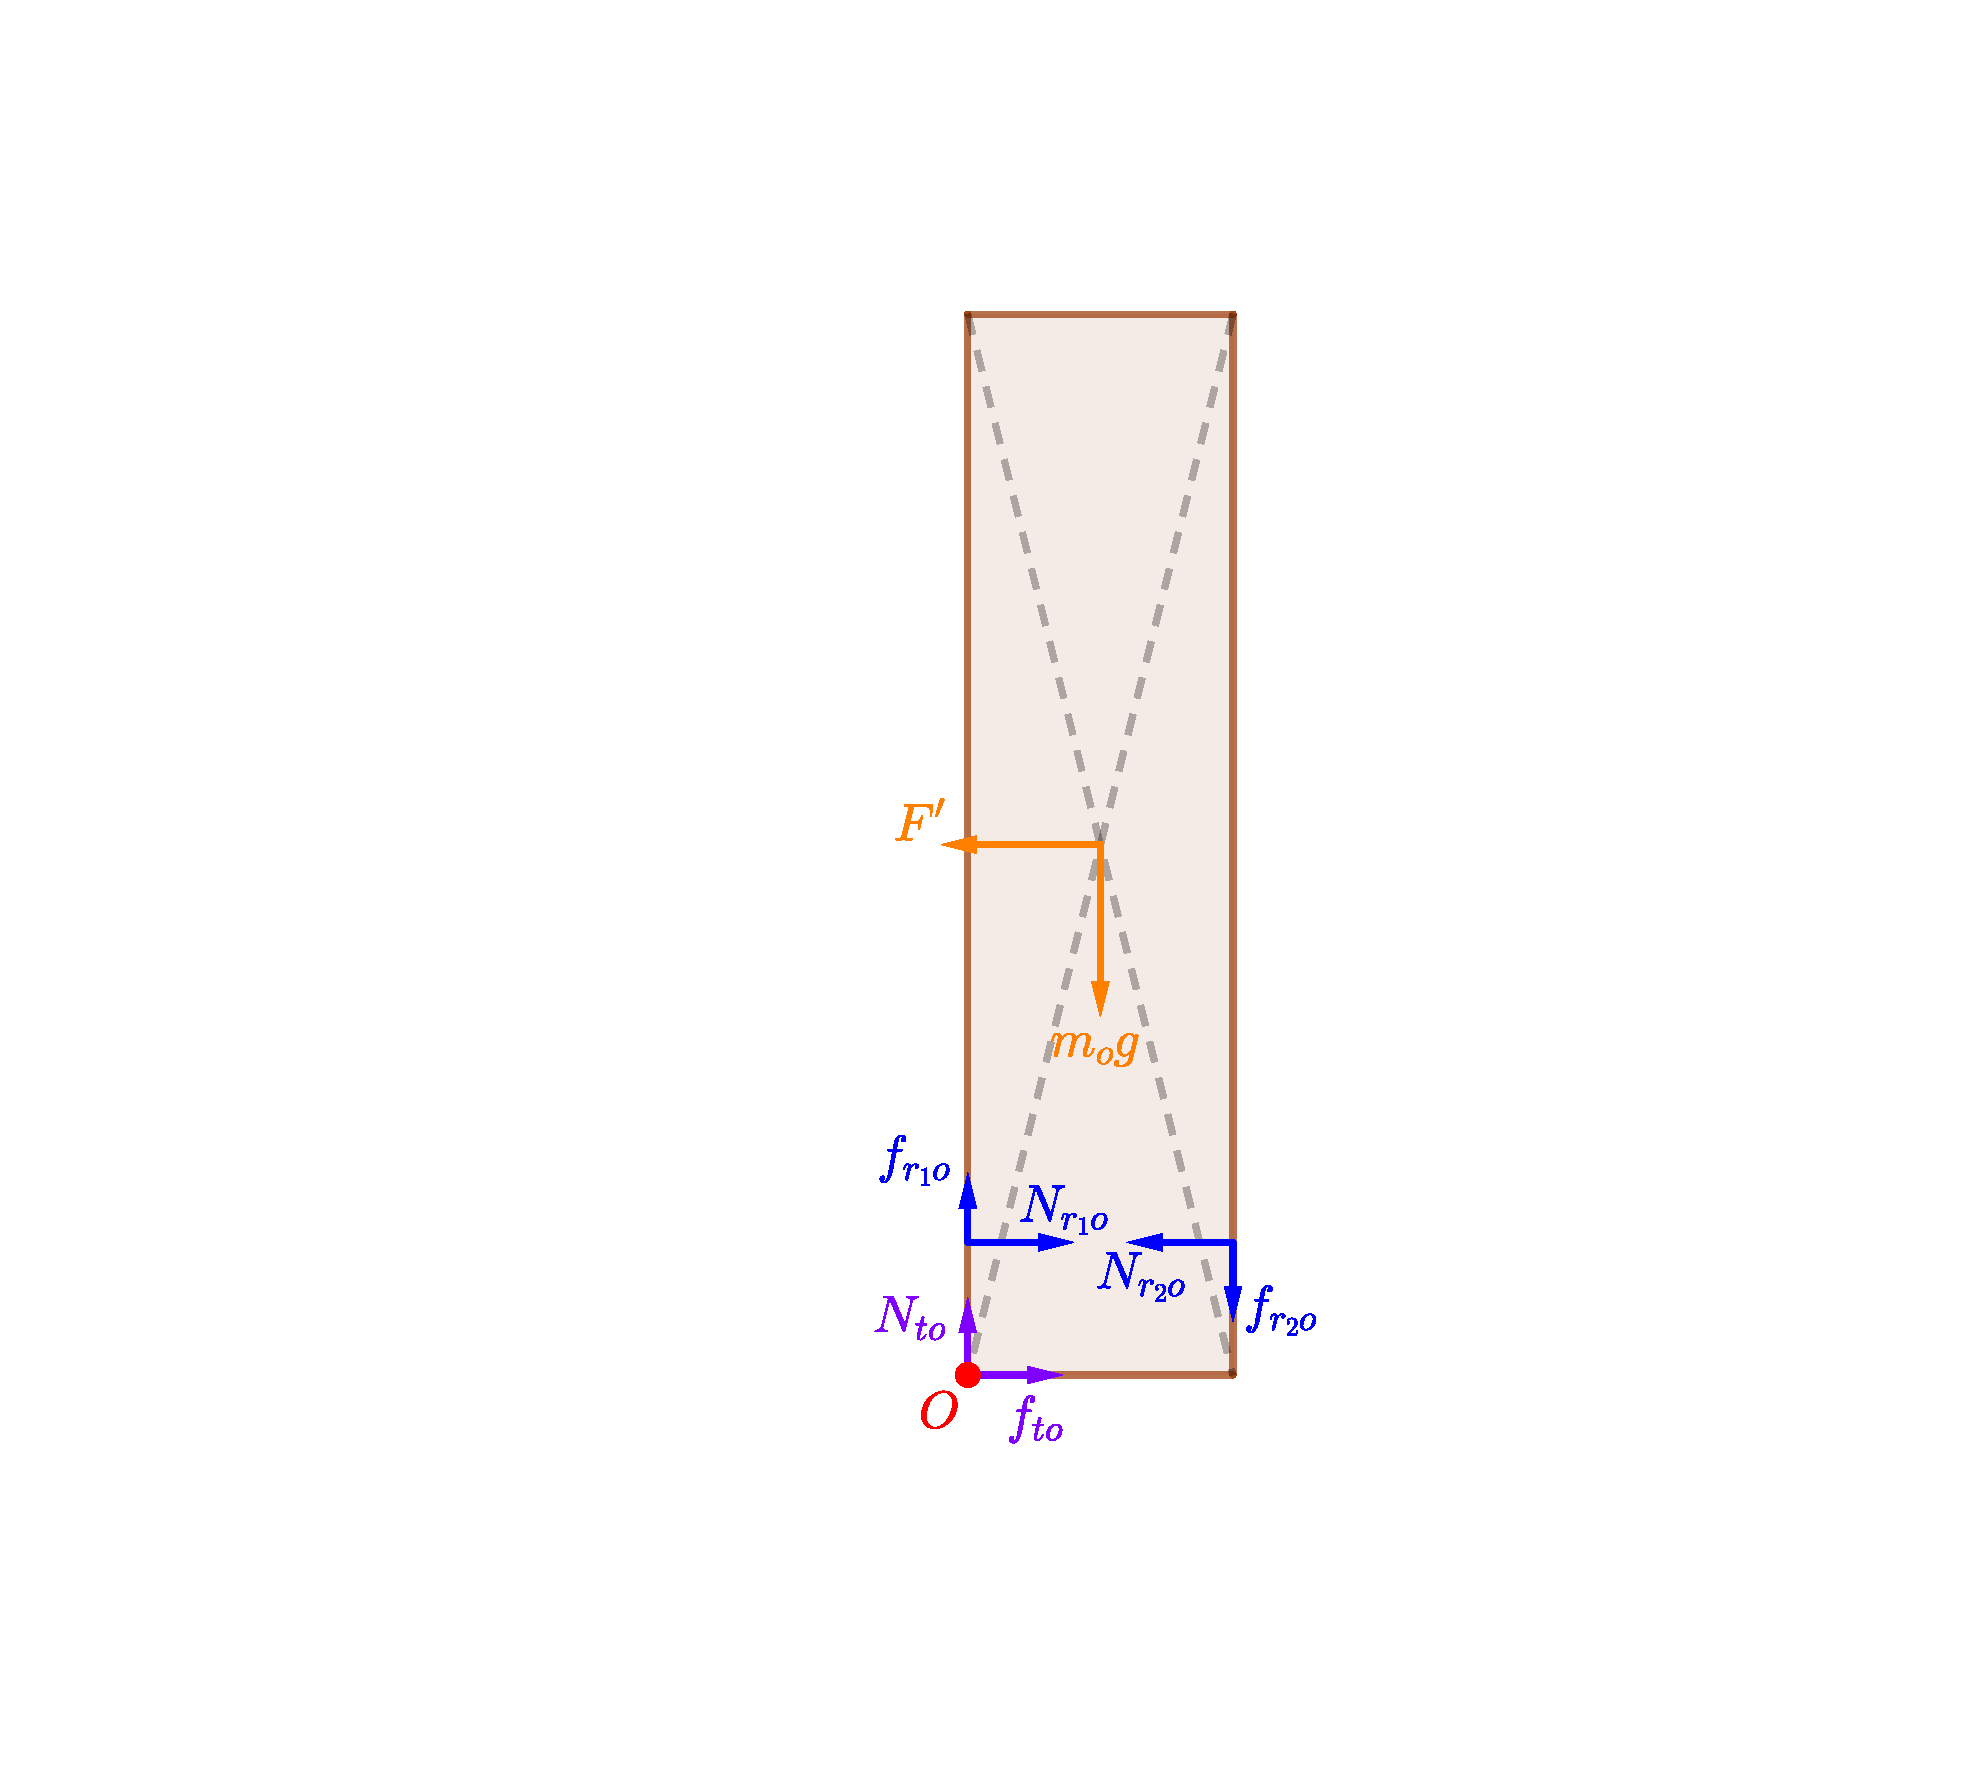
\includegraphics[width=0.5\columnwidth]{./figure/freebody.pdf}
     \caption{Free body diagram of object}
     \labfig{freebody}
   \end{minipage}
  \end{tabular}
\end{figure}

\begin{table}[b]
\caption{Parameters of model}
\centering
\begin{tabular}{c|c}
\hline
Parameter & Description                   \\ \hline\hline
$b_o$       & Width of object              \\ \hline
$h_o$      & Height of object               \\ \hline
$h_r$      & Height of robot               \\ \hline
$m_o$     & Mass of object        \\ \hline
$f_{r_1 o}$       & Friction from robot1 acting on object                 \\ \hline
$f_{r_2 o}$ & Friction from robot2 acting on object                 \\ \hline
$f_{t o}$ & Friction from trolley acting on object                 \\ \hline
$N_{t o}$ & Normal force from trolley acting on object                 \\ \hline
$N_{r_1 o}$ & Normal force from robot1 acting on object                 \\ \hline
$N_{r_2 o}$ & Normal force from robot2 acting on object                 \\ \hline
\end{tabular}
\label{tab:model-parameter}
\end{table}

次に,物体が傾き始めるの台車にかけるための右向きの力を調べる.ここで,物体が傾き始める条件は台車からの垂直抗力の作用点と回転軸の一致である.この条件のもとに,\reffig{freebody}に示すような物体に働く全ての力についての点$O$まわりのモーメントの釣り合いの式を立てたものが\eqref{equilibrium}式である.
\begin{equation}
F^{\prime} \frac{h_{o}}{2}+N_{r_{2} o} \frac{h_{r}}{2}=m_{o} g \frac{b_{o}}{2}+N_{r_{1} o} \frac{h_{r}}{2}+f_{r_{2} o} b_{o}
\label{equilibrium}
\end{equation}
\eqref{equilibrium}式より,
物体が傾き始めるときの台車にかかる力$F^{\prime}$について解くと,\eqref{F-solve}式になる.
\begin{equation}
    F_{\text { topple }}=\frac{h_{r}}{h_{o}}\left(N_{r_{1} o}-N_{r_{2} o}\right)+\frac{b_{o}}{h_{o}}\left(m_{o} g+2 f_{r_2 o}\right)
    \label{F-solve}
\end{equation}
また,ロボットからの垂直抗力$N_{ro}$をロボットの前進力$F_{r}$とロボットと台車の間の摩擦力$f_{tr}$で表現すると,
\begin{equation}
    F_{\text { topple }}=\frac{h_{r}}{h_{o}}\left(F_{r_{1}}-F_{r_{2}}+f_{t{r_1}}+f_{t{r_2}}\right)+\frac{b_{o}}{h_{o}}\left(m_{o} g+2 f_{r_2 o}\right)
    \label{F-solve-again}
\end{equation}
になる.
ただし,物体の左にあるロボット1の前進力$F_{r_{1}}$は右方向に働く.一方,物体の右にあるロボット2の前進力$F_{r_{2}}$は左方向に働く.
ここで,\eqref{F-solve-again}式より,物体が傾き始めるの台車にかけるための力$F_{\text { topple }}$を大きくするためつまり,物体をより安定に支持するための条件を以下にまとめる.
\begin{enumerate}
    \item 1項目のロボットと物体の高さの比$\frac{h_{r}}{h_{o}}$を大きくする.
    \item 1項目のロボット1とロボット2の前進力の差$F_{r_{1}}-F_{r_{2}}$を大きくする.
    \item 1項目のロボットと台車の間の摩擦$f_{t{r_1}}+f_{t{r_2}}$を大きくする.
    \item 2項目の物体の幅と高さの比$\frac{b_{o}}{h_{o}}$を大きくする.
    \item 2項目の物体の質量$m_{o}$を大きくする.
    \item 2項目のロボット2と物体との摩擦$f_{r_2 o}$を大きくする.  
\end{enumerate}
上に述べた条件の中で,1,4,5は既定で,2,3,6が可変なパラメータである.ここで筆者はロボットと台車の間の摩擦に注目した.すなわち,上下のロボット同士の間の摩擦をできるだけ大きくすることを目標に実機の開発を行う.

% \[
% F_{\text { topple }(O_2)}=\frac{1}{h_{o}-2 h_{r}}\left[h_{r}\left(N_{r_{2} o}-N_{r_{1} o}+2 f_{t o}\right)+b_{o}\left(m_{o} g+2 f_{r_2 o}\right)\right]
% \]

%\section{シミュレーション概要}
